\documentclass[output=paper,colorlinks,citecolor=brown]{langscibook}
\ChapterDOI{10.5281/zenodo.14266335}
\author{Stavros Skopeteas\orcid{0000-0002-2827-0518}\affiliation{University of Göttingen}}
\title{Post-predicate prosody in OV languages}

\abstract{This article examines the prosodic properties of post-predicate material in OV languages of the Western Asian Transition Zone. The core question is whether the right edge of the predicate is associated with the edge of a prosodic domain. The facts reported for these languages are summarized in two major phenomena that reveal an asymmetry between the material at the left and right side of the predicate. In some languages (e.g., in Standard Turkish), the nuclear stress must be realized within the domain preceding the right edge of the predicate, that is the pre-predicate material or the predicate itself. In some languages (e.g., in Georgian), the post-predicate material is separated from the predicate with a prosodic event that demarcates a prosodic constituent. Both phenomena provide evidence for a syntactic constituent that is mapped on prosody and separates the post-predicate elements from the core clause.
}

%move the following commands to the "local..." files of the master project when integrating this chapter
% \usepackage{tabularx}
% \usepackage{langsci-optional}
% \usepackage{langsci-gb4e}
% \usepackage{graphicx}
% \usepackage{tikz}
% \bibliography{localbibliography}
% \newcommand{\orcid}[1]{}
% \let\eachwordone=\itshape

\IfFileExists{../localcommands.tex}{
   \addbibresource{../localbibliography.bib}
   \addbibresource{../collection_tmp.bib}
   \bibliography{../localbibliography}
   \usepackage{langsci-optional}
\usepackage{langsci-gb4e}
\usepackage{langsci-lgr}

\usepackage{listings}
\lstset{basicstyle=\ttfamily,tabsize=2,breaklines=true}

%added by author
% \usepackage{tipa}
\usepackage{multirow}
\graphicspath{{figures/}}
\usepackage{langsci-branding}

   
\newcommand{\sent}{\enumsentence}
\newcommand{\sents}{\eenumsentence}
\let\citeasnoun\citet

\renewcommand{\lsCoverTitleFont}[1]{\sffamily\addfontfeatures{Scale=MatchUppercase}\fontsize{44pt}{16mm}\selectfont #1}
  
   %% hyphenation points for line breaks
%% Normally, automatic hyphenation in LaTeX is very good
%% If a word is mis-hyphenated, add it to this file
%%
%% add information to TeX file before \begin{document} with:
%% %% hyphenation points for line breaks
%% Normally, automatic hyphenation in LaTeX is very good
%% If a word is mis-hyphenated, add it to this file
%%
%% add information to TeX file before \begin{document} with:
%% %% hyphenation points for line breaks
%% Normally, automatic hyphenation in LaTeX is very good
%% If a word is mis-hyphenated, add it to this file
%%
%% add information to TeX file before \begin{document} with:
%% \include{localhyphenation}
\hyphenation{
affri-ca-te
affri-ca-tes
an-no-tated
com-ple-ments
com-po-si-tio-na-li-ty
non-com-po-si-tio-na-li-ty
Gon-zá-lez
out-side
Ri-chárd
se-man-tics
STREU-SLE
Tie-de-mann
}
\hyphenation{
affri-ca-te
affri-ca-tes
an-no-tated
com-ple-ments
com-po-si-tio-na-li-ty
non-com-po-si-tio-na-li-ty
Gon-zá-lez
out-side
Ri-chárd
se-man-tics
STREU-SLE
Tie-de-mann
}
\hyphenation{
affri-ca-te
affri-ca-tes
an-no-tated
com-ple-ments
com-po-si-tio-na-li-ty
non-com-po-si-tio-na-li-ty
Gon-zá-lez
out-side
Ri-chárd
se-man-tics
STREU-SLE
Tie-de-mann
}
%    \boolfalse{bookcompile}
%    \togglepaper[1]%%chapternumber
}{}
\begin{document}
\maketitle\label{WOWA:ch:3}

\section{Introduction}\label{sec:intro}
In a study on the punctuation of the Georgian\il{Kartvelian!Georgian} translation of the \textit{Physiologus} (11th c. CE), \citet{boeder_phrasing_1991} reports that scribes often used punctuation within clauses indicating – or possibly prescribing – the prosodic phrasing of subclausal units. The use of punctuation in this manuscript revealed an interesting asymmetry between material at the left and the right side of the verb: setting clitics aside, arguments or adjuncts following the verb were often separated by punctuation, as indicated by the colon in (\ref{ex:oldGeorgian}), but this did not apply when the same elements appeared preverbally.


\newpage
\ea \label{ex:oldGeorgian}
    Old Georgian \il{Kartvelian!Georgian (Old)}(\textit{Physiologus} 6.177.29, edited by \citealt{marr_fisiolog_1904}; cited from \citealt{boeder_phrasing_1991}) \\
    \gll \textit{da} \textit{sameupo-s} \textit{i-ṗov-eb-in} : \textit{kalandr-i} \textit{igi}\\
    and	realm-\textsc{nom}	\textsc{pass}-[\textsc{3sg}]find-\textsc{sm}-\textsc{pass} {} charadrius-\textsc{nom}	\textsc{dem}.\textsc{rem}\\
\glt `and it is found in the realm, that charadrius (bird).'
\z

% \setlength{\footheight}{49.46017pt}
\largerpage

The asymmetry between the left and the right side of the predicate, as reported in \citet{boeder_phrasing_1991}, opens an interesting agenda: is there a difference between pre-predicate and post-predicate elements regarding their prosodic properties? Under which conditions does the post-predicate material appear outside the phonological domain that contains the predicate?  In particular for languages with \isi{OV} properties, a reasonable hypothesis is that the prosodic separation of the post-predicate domain may reflect properties of a predicate-final constituent structure. In many languages, prosodic structure is used for the demarcation information structural domains. At the empirical side, the challenge is to disentangle effects of constituent structure and effects on \isi{information structure}. At the analytical side, the interesting question is whether the information structural options of a language can be partially predicted from the array of possible prosodic structures in this language.

In order to tackle these questions, the present study examines selected \isi{OV} languages of the Western Asian Transition Zone, which comprises the area of Northern Iran, Northern Iraq, Eastern Turkey and the Caucasus  \citep[350]{Stilo2015AIAtlas}{}; see Chapter 1, this vol. The languages in this area are not syntactically uniform, but most languages generally share several ``\isi{OV}'' properties, such as preverbal placement of bare objects and auxiliaries following the lexical verb, which at least distinguish them from \isi{VO} languages. The contextual conditions of \isi{OV} and \isi{VO} differs very much between languages, as established by various studies (\citealt[]{stilo_preverbal_2018}, \citealt{haig_which_2023}, Chapter 1, this vol.), which will be one of the main issues in the following discussion (see \sectref{sec:focusOptions}).

\largerpage
The primary data discussed in the present study was elicited with native speakers of Turkish\il{Turkic!Turkish}, Georgian\il{Kartvelian!Georgian}, Caucasian Urum\il{Turkic!Caucasian Urum}, Eastern Armenian\il{Armenian (Eastern)}, and Persian\il{Persian}. The aim of this elicitation was to obtain comparable data that illustrate the phenomena at issue; however, the main source of the discussed generalizations is the available research on these languages.\footnote{The data were collected in qualitative interviews with native speakers, who were raised in the \isi{object} language and currently use it in their everyday life. Beyond their native language, these speakers were also competent in English\il{English} or German\il{German}. The Caucasian Urum\il{Turkic!Caucasian Urum} speaker was also native in Russian\il{Russian} and Georgian\il{Kartvelian!Georgian}; the further speakers did not speak other languages of the area. The speakers prepared the sentences in collaboration with the instructor and were instructed to imagine a conversation in which the scripted utterances are performed as answers to context questions. They were free to repeat their performance until they were confident that it corresponds to a natural way to produce the target utterance in the given context.} Information about further languages
of this area is drawn from the available research. The majority of the available sources is based on controlled data, either scripted speech or controlled speech-production tasks. This method comes with limitations in the generalizability of the findings, which should not be neglected. 

Based on the available comparisons between spontaneous and controlled data in the phenomena under consideration, the major issue is that elicited data may present ``idealizations'' of what happens in real discourse. A comparison between scripted speech and semi-spontaneous narratives in Georgian\il{Kartvelian!Georgian} reports that post-predicate elements are often separated by a high prosodic boundary from the predicate in either type of data: spontaneous narratives differ from controlled speech in that they display greater variability \citep[44]{Skopeteasetal_Information_2018}. This means that controlled data present an ``idealization'' of patterns that are learnt in real life \citep{stokhof_abstractions_2011}. Idealization of phonological events may have the form of hyper-articulation, e.g., expansion of the pitch range of tonal events that are less salient in spontaneous speech. In a study on Persian\il{Persian}, spontaneous data were found to be often under-specified in comparison to controlled data: since prosodic demarcation is often not necessary for conveying the intended content, it is expected that real communication will be less rich in prosodic marking than the performance in careful speech \citep[28--31]{sadat-tehrani_intonation_2017}. Finally, the difference does not only lie in the clarity of signaling a certain \isi{information structure}, but also in the intention of the speaker to convey the \isi{information structure} of the utterance or not. Information structure is not an automatic reflex of the context, which often results in discrepancies between the intuitions of the speakers and what we find in corpora. For instance, \citet[243]{forker_word_2016} report that some speakers of Tsakhur do not accept postverbal objects in narrow \isi{focus} (with reference to \citealt[]{testelec_porjadok_1999}), but postverbal objects appear in Tsakhur texts as answers to questions that license a narrow \isi{focus} on the \isi{object}. This discrepancy may have two explanations: (a) the speakers report wrong generalizations about their native language; (b) since the \isi{information structure} of the answer is made clear through the context, an answer that does not necessarily mark narrow \isi{focus} is fully adequate in view of the communicative goals. Hence, these cases involve the challenge of identifying the intention of the speaker in producing an utterance in a certain context. This is not trivial of course, but it is relevant for the interpretation of the facts -- if we do not assume that the relation between context and target utterance is deterministic. Finally, either type of speech production may be influenced by phenomena that are not related to the matter at issue: scripted speech may be performed with listing \isi{intonation} (i.e., continuation rises at the end of declarative clauses), if the native speakers are not instructed to realize the utterances as complete discourse units; spontaneous data often show reflexes of speech planning, e.g., hesitation pauses, which lead to shorter intonational units than in controlled settings \citep[31-33]{sadat-tehrani_intonation_2017}.

With this background, the goal of the present study is to identify prosodic properties of post-predicate elements in the available data and to set up hypotheses about their relation to syntax and/or \isi{information structure}. The properties of post-predicate elements are not uniform across constructions: at least in many Iranian languages, the verb governs direct objects on its left and \isi{oblique} objects (especially \isi{Goal} arguments) on its right side, as it has been demonstrated with rich data in \citet{HaigRasekhMahand2019}, \citet{haig_which_2023}, and \textcitetv{chapters/7_RasekhMahandetal_Persian}. This difference is also reflected in the \isi{focus} options and prosodic properties of the different classes of complements \citep[138--139]{sadat-tehrani_intonational_2007}, which means that post-predicate elements form different types of domains with the predicate, which are also reflected in \isi{prosody}. In order to restrict the sources of variation, we will only examine preverbal and postverbal direct objects in the present study.

The following exposition starts with an overview of the variation between languages in the \isi{information structure} of post-predicate objects; see \sectref{sec:focusOptions}. After a short summary of the necessary assumptions for prosodic description in \sectref{sec:assumptions}, the core part of the study is organized around the \isi{information structure} of post-predicate objects. The basic distinction is whether the post-predicate \isi{object} is part of the partition of the utterance that is focused (i.e., the \isi{focus} domain) or not. In the former case, it can be part of a larger \isi{focus} domain that contains the post-predicate and the predicate: these are instances of ``broad focus\is{focus!broad},'' that may contain a VP or an entire sentence (see \sectref{sec:broad}). Alternatively, the \isi{focus} domain of the utterance may be exactly the post-predicate \isi{object}; these are cases of ``narrow \isi{focus}'' (i.e., a \isi{focus} domain only containing a simple lexical projection such as a noun phrase) (see \sectref{sec:narrow}). Finally, the post-predicate \isi{object} may be outside the \isi{focus} domain (or simply ``out of \isi{focus}''), in which case it is background information (see \sectref{sec:out}). Based on the properties introduced in these sections, \sectref{sec:summary} draws conclusions about the interaction between syntax and \isi{prosody} in the realization of post-predicate elements.

\newpage
\section{Focus options} \label{sec:focusOptions}
\largerpage[-1]
V-final languages of the Western Asian Transition Zone differ regarding the \isi{focus} possibilities of post-predicate objects. They either cannot be focused (Turkish), or they can be part of a narrow/broad focus\is{focus!broad} domain (Georgian) or of a broad focus\is{focus!broad} domain only (Persian). 

Post-predicate elements in Modern Standard Turkish\il{Turkic!Turkish} can be either background information (discourse given information that is outside the \isi{focus} domain of the utterance) or afterthoughts (discourse new information that completes the utterance) (see \citealt[50--56]{taylan_function_1984}, \citealt[]{issever_information_2003}, \citealt[727-728]{kilicaslan_syntax_2004}). Afterthoughts are a different type of phenomenon since they were not part of the sentence plan at the critical time point that the speaker selected the linearization of her utterance. Leaving afterthoughts aside, post-predicate elements in this type of language cannot be focused. This phenomenon is reported for Western Armenian\il{Armenian (Western)} \citep[§2.7]{donabedian-demopoulos_middle_2018}, Laz\il{Kartvelian!Laz} \citep[852]{lacroix_laz_2018}, and Balochi \citep[66-68]{delforooz_discourse_2010}. Northwest Caucasian languages presumably belong to this group as well -- at least those languages like Ubykh in which postverbal constituents are rare \citep[977]{forker_information_2021}.

In a second type of languages, post-predicate objects are contextually unrestricted. In Georgian\il{Kartvelian!Georgian}, postverbal objects can be either part of a broad focus\is{focus!broad} (e.g., a \isi{focus} domain encompassing the entire clause) or a narrow \isi{focus} (e.g., \isi{focus} on the postverbal \isi{object}) (\citealt[]{skopeteas_Fanselow_focus_2010}, \citealt[170]{gosby_information_2016}, \citealt[106, 235]{borise_phrasing_2019}, Chapter 10, this vol.). Similar facts are reported for Mingrelian and Svan \citep[994]{forker_information_2021}, Caucasian Urum\il{Turkic!Caucasian Urum} \citep[221]{schroter_information_2017}, Ossetic\il{Ossetic} \citep[686]{erschler_preverbal_2012}, and at least some Nakh-Daghestanian languages (see summary in \citealt[977]{forker_information_2021}). In Eastern Armenian\il{Armenian (Eastern)}, the same flexibility of the post-predicate domain applies to synthetic verbs (in \isi{contrast} to periphrastic verbs, in which case the \isi{auxiliary} cliticizes to the element bearing the nuclear stress, such that the material following the \isi{auxiliary} is de-accented (\citealt[]{comrie_formal_1984}, \citealt[]{kahnemuyipour_second_2011}, \citealt[]{samvelian_persistence_2023}).  

The difference between languages with and languages without postverbal foci is well established in the research on V-final languages. Interestingly, there is a third pattern that deserves more attention. \citet[243]{forker_word_2016} (with reference to \citealt[]{testelec_porjadok_1999}) report that some speakers of Tsakhur accept postverbal objects in broad focus\is{focus!broad}, but not so in narrow \isi{focus}. A similar asymmetry is gathered through speaker judgments in Persian\il{Persian}: \textit{specific} objects can follow the predicate when they are part of a broad focus\is{focus!broad} domain, but they are judged to be impossible in narrow \isi{focus} (see \citealt[115]{karimi_object_2003} and \citealt[68, 138--139]{sadat-tehrani_intonational_2007} for the latter statement); see (\ref{ex:Persian})\footnote{These intuitions imply that speakers will use a preverbal \isi{object} whenever they intend to signal that this constituent is narrowly focused. The prediction for corpus observations is that preverbal objects are \textit{more likely} in contexts licensing a narrow \isi{focus} on the \isi{object} than in contexts licensing a broader \isi{focus} domain including the \isi{object} (assuming that a subset of the data from speech production are under-specified for \isi{information structure}). The only corpus study that offers data for this comparison is a small-size corpus study on written Persian\il{Persian}, showing that \isi{SVO} appears rarely in sentence/predicate \isi{focus} and never in narrow \isi{focus} \citep[861]{majidi_information_2012} -- but the size of the corpus does not allow for strong statements. The corpus study by \citet[139--141]{roberts_study_2009} on written/oral Persian\il{Persian} shows that postverbal specific objects may be part of the \isi{focus} domain, but does not consider instances of narrow \isi{focus}. \citet[243]{forker_word_2016} present examples with postverbal objects in Tsakhur that are answers to questions licensing a narrow \isi{focus} on the \isi{object}, which contradict the speakers' intuitions, but without excluding that these answers are underspecified for \isi{information structure} since this is clearly indicated by the context (see discussion in \sectref{sec:intro}).}

\begin{samepage}
\ea \label{ex:Persian}
    Persian \il{Persian}(Y. Sanei, p.c.) \\ 
    \ea Broad \isi{focus} (entire clause)\\
    A: ‘What happened?’\\ 
    \gll \textup{B:} \textit{Nâzanin} \textit{livân-am-o} \textit{var-dâšt}.\\
         ~ Nazanin glass-\textsc{poss.1sg}-\textsc{ra} up-have:\textsc{pst}[\textsc{3sg}]\\
    \glt \hspace{0.4cm}‘Nazanin picked up my glass.’\\
    \gll  \textup{B´:} \textit{Nâzanin} \textit{var-dâšt} \textit{livân-am-o}.\\
        ~ Nazanin up-have:\textsc{pst}[\textsc{3sg}] glass-\textsc{poss.1sg}-\textsc{ra}\\
    \glt \hspace{0.5cm}‘Nazanin picked up my glass.’
    \ex Narrow \isi{focus} (on the \isi{object})\\
        A: ‘What did Nazanin pick up?’\\
        B: \textit{Nâzanin livân-am-o var-dâšt}.\\
        B´: \#\textit{Nâzanin var-dâšt livân-am-o}.\\
    \z
\z
\end{samepage}    

\begin{sloppypar}
\isi{OV} languages of this region share some properties in this respect. First, postverbal arguments can be background information. Furthermore, in all these languages there is evidence for a preverbal position for narrow \isi{focus}, which is immediately left adjacent to the verb: Turkish\il{Turkic!Turkish} \citep[]{goksel_is_2000}, Laz\il{Kartvelian!Laz} \citep[852]{lacroix_laz_2018}, Georgian\il{Kartvelian!Georgian} \citep[235]{borise_phrasing_2019}, Chechen\il{Caucasian (East)!Chechen} \citep[322]{komen_finding_2013}{},  Nakh-Daghestanian (in general)  \citep[977]{forker_information_2021}, Northwest Caucasian (in general) \citep[986]{forker_information_2021}, Ossetic\il{Ossetic} (\citealt[686]{erschler_preverbal_2012}, \citealt[]{borise_flexible_2023}), Eastern Armenian\il{Armenian (Eastern)} (\citealt[19]{comrie_formal_1984}, \citealt[464--467]{samvelian_persistence_2023}), Persian\il{Persian} \citep[]{kahnemuyipour_wh-questions_2001}. Beyond the preverbal option, there is a lot of variation regarding the exact \isi{focus} options in the preverbal domain, e.g., whether the preverbal elements can be marked for \isi{focus} in their canonical position, whether contrastive foci may have an effect on linear order, as in Persian\il{Persian} \citep[92]{karimi_object_2003}, which is out of the scope of the present study. In \isi{contrast} to preverbal foci, postverbal foci are not restricted to a certain position that is designated to \isi{focus}: any element within the post-predicate domain can be focused by prosodic means.
\end{sloppypar}

The language types presented so far are summarized in \figref{fig:treeIS}. The first node contains the already established distinction between languages in which the post-predicate domain cannot be focused and languages allowing for \isi{focus} on post-predicate elements. Within the latter type, there is a distinction between languages that allow for any type of \isi{focus} and those that only allow for broad focus\is{focus!broad} in the post-predicate domain.

\begin{figure}
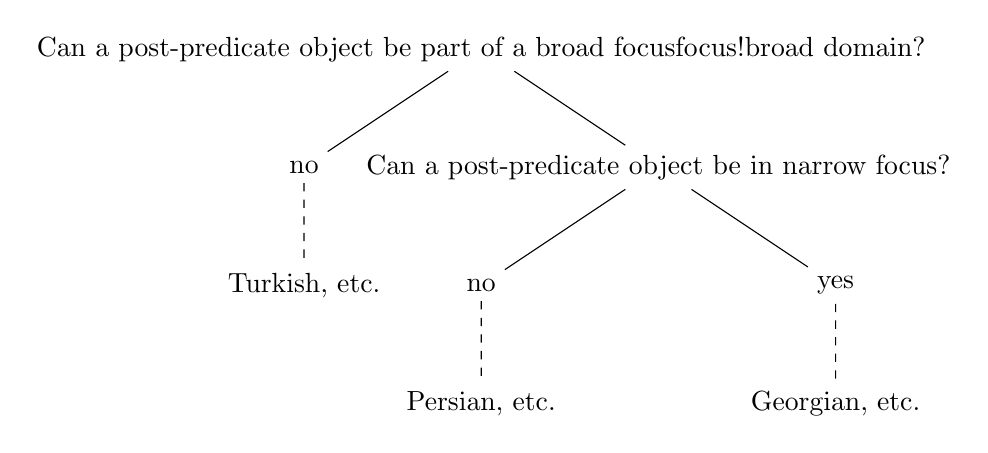
\begin{tikzpicture}
    \node {Can a post-predicate \isi{object} be part of a broad focus\is{focus!broad} domain?}[sibling distance = 4.5cm]
    child {node {no}
    child {node {Turkish, etc.} edge from parent [dashed]}}
    child {node {Can a post-predicate \isi{object} be in narrow \isi{focus}?}
    child {node {no}
    child {node {Persian, etc.} edge from parent [dashed]}}
    child {node {yes}
    child {node {Georgian, etc.} edge from parent [dashed]}} 
};
\end{tikzpicture}
\caption{Focus options of post-predicate objects in OV languages of the Western Asian Transition Zone}
    \label{fig:treeIS}
\end{figure}

Note that \figref{fig:treeIS} reveals an implicative relation between the \isi{focus} options of post-predicate objects, since no language in this sample expresses narrow but not broad focus\is{focus!broad} in the post-predicate domain (see \ref{ex:implication}).

\ea \label{ex:implication}
    Between \isi{focus} options of post-predicate objects\\
    Broad \isi{focus} ← Narrow \isi{focus}\\
\z

The origin of this asymmetry will be discussed in \sectref{sec:outlookFocusoptions} in the light of the prosodic properties of the languages at issue, which are examined in the subsequent sections.

\section{Prosodic assumptions} \label{sec:assumptions}

\begin{sloppypar}
The description of the collected data in the following sections is built upon some basic assumptions about the relevant prosodic events and the syntax-\isi{prosody} interface, that are introduced in the following. Prosodic constituents form a prosodic hierarchy such that constituents of higher layers optionally contain constituents of lower layers. The correspondence between prosodic constituents and syntactic constituents is roughly as follows: prosodic words (ω) correspond to morphological words including clitics; phonological phrases (φ) correspond to syntactic phrases; \isi{intonation} phrases (ι) to clauses \citep[437]{selkirk_syntax-phonology_2011}. These correspondences are modulated by purely phonological rules (e.g., constraints on the size of prosodic constituents), by other functions reflected in prosodic phrasing (e.g., \isi{focus}) and by aspects relating to speech performance, such as speech tempo and hesitation breaks. For instance, the expression of \isi{focus} may create prosodic constituents that do not correspond to syntactic phrases; see (SV)\textsubscript{φ} in example (\ref{ex:urumNarrow}b) below. We assume that prosodic constituents allow for recursion, such that φ-phrases can be embedded in other φ-phrases as in (α (β)\textsubscript{φ})\textsubscript{φ} (see discussion in \citealt[]{ladd_intonational_1986}, \citealt[455]{selkirk_syntax-phonology_2011}, \citealt[78--85]{fery_intonation_2018}).
\end{sloppypar}

The pitch track annotations in the following examples follow the conventions of the Autosegmental-Metrical framework \citep[]{pierrehumbert_phonology_1980}. Tonal events represent the assumed phonological entities that underlie the pitch contour -- and not every peak or dip in the pitch excursion. The labels indicate the scaling of tonal targets with respect to their environment (H for ‘high’, L for ‘low’, L+H for ‘rise’, etc.), and for their association with two classes of entities: (a) edge tones are associated with the edges of prosodic constituents (H\textsubscript{φ}: is a high tone associated with the right edge of a φ-phrase, \textsubscript{φ}H is a high tone associated with the left edge of a φ-phrase) and (b) pitch accents are associated with stressed syllables (H* is a high tone associated with the stressed syllable; L+H* is a rise, whose H-target is associated with the stressed syllable). Languages often mark the constituent that hosts the nuclear stress of the \isi{intonation phrase} (i.e., the constituent that is perceived with maximal prominence) with different tonal events from the prosodic constituents that precede or follow it (``prenuclear'' or ``postnuclear'' prosodic constituents).

The phonetic cues of prosodic constituents are language specific. Prosodic constituents may be demarcated by tonal events or breaks at their edges as well as by effects on the duration of edge syllables (e.g., final lengthening). Further evidence for prosodic constituents comes from \isi{register} lowering: the pitch scaling of tonal events at sister constituents incrementally decreases (\citealt[]{ladd_declination_1988}, \citealt[]{fery_focus_2013}). 

\section{Broad focus} \label{sec:broad}

A broad focus\is{focus!broad} encompassing the entire utterance is elicited with a context question that does not introduce any presuppositions, such as ‘What happened?’. \figref{fig:georgianBroad} illustrates the \isi{contrast} between the SOV and the \isi{SVO} order in this context in Georgian\il{Kartvelian!Georgian}. The SOV utterance (\textsc{Left Panel}) is realized with a series of rising contours (\textsubscript{φ}L...H\textsubscript{φ}), stretching from a low target at the left edge to a high target at the right edge of the φ-phrase (see various analyses in \citealt[]{skopeteas_word_2009}, \citealt[]{vicenik_autosegmental-metrical_2014}, \citealt[]{Skopeteasetal_Information_2018}, \citealt[]{borise_focus_2021}). The second H\textsubscript{φ} is scaled lower than the first H\textsubscript{φ}. The final verb is realized with low intensity and creaky voice, which results to a fragmentary pitch signal and ends with a final lowering, represented by the L target at the right edge of the ι-phrase (L\textsubscript{ι}). The \isi{SVO} realization (\textsc{Right Panel}) differs (see detailed discussion in \citealt[]{skopeteas_Fery_focus_2010}, \citealt[]{Skopeteasetal_Information_2018}): the subject and the verb are integrated in a single phonological domain that is determined by a \textsubscript{φ}H tone at the left edge and a H\textsubscript{φ} tone at the right edge. Crucially, the latter phrase tone is not lowered with reference to the former one. \footnote{The figures in this article contain an oscillogram (\textsc{Top}) and a track of the f\textsc{0} (\textsc{Middle}) temporally aligned with the phonetic transcription of the utterance (\textsc{Bottom}); created in Praat \citep{boersma_praat_2023}.}

\begin{figure}
    \includegraphics[scale=0.3]{pitch_tracks/GEO-SOV-A}
    \includegraphics[scale=0.3]{pitch_tracks/GEO-SVO-A}
    \caption{Broad focus in Georgian\il{Kartvelian!Georgian}; answers to ‘What happened?’, \textsc{Left Panel}: SOV; \textsc{Right Panel}: SVO; morphemic transcription in (\ref{ex:georgianBroadSOV})-(\ref{ex:georgianBroadSVO})}
    \label{fig:georgianBroad}
\end{figure}

 The \isi{register} lowering of the second H-target in the SOV order (\figref{fig:georgianBroad}/\textsc{Left Panel}) is compatible with two alternative analyses, see (\ref{ex:georgianBroadSOV}): (a) the H-targets can be associated with the right edge of two sister φ-phrases that are mapped onto the preverbal arguments; (b) alternatively, the second φ-phrase can be associated with a φ-phrase mapped onto the \isi{object}, that is nested within the φ-phrase of the VP. Register lowering applies to this case too, since the φ-phrase of the VP is a sister constituent to the φ-phrase of the subject. Hence, both prosodic structures in (\ref{ex:georgianBroadSOV}) are possible and the realization of the example does not provide any further cues that would support the one or the other structure.

\ea \label{ex:georgianBroadSOV}
    Georgian \il{Kartvelian!Georgian}(D. Kakashvili, p.c.) \\
    \gllll \textup{\textsubscript{φ}L} \textup{H\textsubscript{φ}} \textup{\textsubscript{φ}L} \textup{H\textsubscript{φ}} {} \textup{L\textsubscript{ι}} \\
    ((\textit{monadire-m}\textsubscript{ω} )\textsubscript{φ} (\textit{melakuda}\textsubscript{ω} )\textsubscript{φ} \textit{da-k’arg-a}\textsubscript{ω} )\textsubscript{ι}\\
    ((\textit{monadire-m}\textsubscript{ω} )\textsubscript{φ} ((\textit{melakuda}\textsubscript{ω} )\textsubscript{φ} \textit{da-k’arg-a}\textsubscript{ω})\textsubscript{φ} )\textsubscript{ι}\\
     hunter-\textsc{erg} ~ fox[\textsc{nom}] ~ \textsc{pfv}-loose-\textsc{aor}.\textsc{s}.\textsc{3sg}\\
\glt ‘The hunter lost the fox.'
\z 

In the \isi{SVO} utterance (\figref{fig:georgianBroad}/\textsc{Right Panel}), the verb and the preverbal material are phrased as a single prosodic constituent. The left edge of this constituent is demarcated with a high phrase tone (\textsubscript{φ}H), while the two phrase tones (\textsubscript{φ}H and H\textsubscript{φ}) are just interpolated. The relevant issue is that the predicate is phrased together with the preceding material and forms a separate prosodic constituent from the post-predicate. Quantitative studies on controlled and spontaneous data show that the high phrase tone at the right edge of the verb is a frequent (but not necessary) correlate of verb-medial orders (\citealt[]{skopeteas_Fery_focus_2010}, \citealt[]{Skopeteasetal_Information_2018}).

\ea \label{ex:georgianBroadSVO}
    Georgian \il{Kartvelian!Georgian}(D. Kakashvili, p.c.) \\
    \glll \textup{\textsubscript{φ}H} ~ \textup{H\textsubscript{φ}} ~ \textup{L\textsubscript{ι}} \\
    ((\textit{monadire-m}\textsubscript{ω} \textit{da-k’arg-a}\textsubscript{ω} )\textsubscript{φ} (\textit{melakuda}\textsubscript{ω})\textsubscript{φ} )\textsubscript{ι}\\
    hunter-\textsc{erg} \textsc{pfv}-loose-\textsc{aor}.\textsc{s}.\textsc{3sg} ~~ fox[\textsc{nom}]\\
\glt ‘The hunter lost the fox.'
\z


The special \isi{role} of the predicate in phrasing is also reported for other languages (see \citealt[771, 780]{borise_tone_2021}{} for a summary of earlier mentions in Adyghe\il{Circassian!Adyghe}, Circassian\il{Circassian}, and Chechen\il{Caucasian (East)!Chechen}; see \citealt[275]{hasan_kurdish_2012} on preverbal and postverbal quotations in Kurmanji\il{Kurdish (Northern)}), but more data is required in order to qualify these reports. However, this phenomenon does not apply to all \isi{OV} languages of the area, as illustrated below for Persian\il{Persian}. 

The available accounts on Persian\il{Persian} \isi{prosody} do not predict a high phrase tone at the right edge of the verb for independent reasons: the nuclear φ-phrase cannot be after the predicate (except for \isi{Goal} arguments) and this phrase normally ends with a low phrase tone \citep[9, 68]{sadat-tehrani_intonational_2007}.\footnote{This does not mean that a high phrase tone at the right edge of the verb is impossible (see an example in \citealt[54]{Mahjani2003}).} Prenuclear φ-phrases are realized with rising contours that reach a H-target within the stressed syllable (i.e., a L+H* pitch accent). This pitch accent is followed by a phrase tone (H\textsubscript{φ}) in prenuclear φ-phrases \citep[9, 42, 68]{sadat-tehrani_intonational_2007} and is tonally compressed or totally erased in postnuclear φ-phrases \citep[]{abolhasanizadeh_persian_2012}. The reflexes of this pitch accent are illustrated in \figref{fig:persianBroad} with specific objects, which may precede or follow the V in Persian\il{Persian}. The L+H* pitch accent is aligned with the stress, which is final with nouns (see \textit{Nâza\textquotesingle nin} `Nazanin') or falls on an earlier syllable in the presence of clitics (see \textit{li\textquotesingle vân-am-o} `glass-\textsc{poss.1sg-ra}') or in the verb complex (see \textit{ne\textquotesingle gâh kard} `look do:\textsc{pst}[\textsc{3sg}]'\footnote{Word
    stress is located on the final syllable of nouns/adjectives with the exception of unstressed enclitics; with complex verbs, the stress falls on the embedded non-verbal element that expresses the lexical content and not on the light verb \citep[]{kahnemuyipour_syntactic_2003}.
}). Prenuclear and nuclear pitch excursions differ with respect to the presence of a H\textsubscript{φ} phrase tone. In prenuclear φ-phrases, the pitch excursion rises up to the right edge of the phrase (see \textit{li\textquotesingle vân-am-o} `glass-\textsc{poss.1sg-ra}' in  the \textsc{Left Panel}); in nuclear φ-phrases, the rising in the stressed syllable (L+H*) is followed by a falling pitch excursion (see \textit{ne\textquotesingle gâh kard} `look do:\textsc{pst}[\textsc{3sg}]' in  the \textsc{Right Panel}), while the postnuclear domain is tonally compressed (\citealt[7--8]{sadat-tehrani_intonational_2007}{}, \citealt[]{taheri_ardali_phonetic_2012}{}). Nuclear rises are scaled lower than prenuclear rises and their H-target (H*) is aligned with the middle of the stressed syllable while the H-target of phrase tones (H\textsubscript{φ}) is aligned with the right edge of the word (\citealt[]{sadat-tehrani_alignment_2009}{}, \citealt[104--107]{hosseini_phonology_2014}{}).


\begin{figure}
    \includegraphics[scale=0.3]{pitch_tracks/PES-SOV-A}
    \includegraphics[scale=0.3]{pitch_tracks/PES-SVO-A}
    \caption{Broad focus in Persian; answers to ‘What happened?’, \textsc{Left Panel}: SOV; \textsc{Right Panel}: SVO; morphemic transcription in (\ref{ex:persianBroad})}
    \label{fig:persianBroad}
\end{figure}

In the SOV order with a specific \isi{object} (\textsc{Left Panel}), the nuclear stress falls on the verb and the φ-phrase of the \isi{object} precedes the nucleus and is enclosed by a H\textsubscript{φ} phrase tone (as expected for specific objects and in \isi{contrast} to bare objects \citep[81]{hosseini_phonology_2014}{}; see (\ref{ex:persianBroad}a)). In the \isi{SVO} order (\textsc{Right Panel}), the nuclear stress is again realized within the verb (as indicated by the absence of a H\textsubscript{φ}), while the post-predicate domain is realized as a low plateau without any tonal events; see (\ref{ex:persianBroad}b). This realization follows from a general property of Persian\il{Persian} \isi{prosody}: (to the exception of \isi{Goal} arguments) the nuclear stress cannot be realized in the domain following the predicate \citep[9, 68]{sadat-tehrani_intonational_2007}. Since the domain of the nuclear stress is the \isi{intonation phrase}, we conclude that the low edge tone is associated with the right edge of an \isi{intonation phrase} (L\textsubscript{ι}).

\begin{samepage}
\ea \label{ex:persianBroad}
    Persian \il{Persian}(Y. Sanei, p.c.) \\ \nopagebreak[4]
    \ea 
    \glll \textup{L\textsubscript{φ}}\hspace{0.4cm}\textup{L+H*} \textup{H\textsubscript{φ}} \hspace{0.3cm}\textup{L+H*} \textup{H\textsubscript{φ}} \hspace{0.4cm}\textup{L+H*} ~ \textup{L\textsubscript{ι}} \\
    ((\textit{nâza\textquotesingle nin}\textsubscript{ω} )\textsubscript{φ} (\textit{li\textquotesingle vân-am-o}\textsubscript{ω} )\textsubscript{φ} (\textit{ne\textquotesingle gâh}\textsubscript{ω} \textit{kard}\textsubscript{ω})\textsubscript{φ} )\textsubscript{ι}\\
            Nazanin ~ glass-\textsc{poss.1sg-ra} ~ look do:\textsc{pst}[\textsc{3sg}]\\
            \glt ‘Nazanin watched my glass.’
    \ex 
        \glll \textup{L\textsubscript{φ}}\hspace{0.5cm}\textup{L+H*} \textup{H\textsubscript{φ}} \hspace{0.4cm}\textup{L+H*} ~ \textup{L\textsubscript{ι}} ~ \textup{L\textsubscript{ι}} \\
            (((\textit{nâza\textquotesingle nin}\textsubscript{ω} )\textsubscript{φ} (\textit{ne\textquotesingle gâh}\textsubscript{ω} \textit{kard}\textsubscript{ω})\textsubscript{φ} )\textsubscript{ι} (\textit{li\textquotesingle vân-am-o}\textsubscript{ω})\textsubscript{φ} )\textsubscript{ι}\\
            Nazanin ~ look do:\textsc{pst}[\textsc{3sg}] ~ glass-\textsc{poss.1sg-ra}\\
        \glt ‘Nazanin watched my glass.’
    \z
\z
\end{samepage}

In sum, the examples of broad focus\is{focus!broad} illustrated two distinct phenomena:
\begin{itemize}
  \item In Georgian\il{Kartvelian!Georgian}, post-predicate objects are prosodically separated from the predicate (by a φ-phrase boundary). 
  \item In Persian\il{Persian}, post-predicate objects are outside the phonological domain (presumably an ι-phrase) that may host the nuclear stress.
\end{itemize}

\section{Narrow focus} \label{sec:narrow}

In some languages, the post-predicate domain can host a narrow \isi{focus} (see \sectref{sec:focusOptions}). Since all these languages also have a preverbal position hosting narrow foci (see \ref{sec:focusOptions}), the relevant question is whether these options differ prosodically. The data presented in this section show that preverbal foci are prosodically integrated to the phonological constituent that contains the verb, while postverbal foci are prosodically separated from verb.

Caucasian Urum\il{Turkic!Caucasian Urum} is an Anatolian dialect of Turkish\il{Turkic!Turkish} spoken by a population that migrated to the Small Caucasus from Kars/Erzurum in the 19th century \citep[]{skopeteas_caucasian_2016}. Similar to the Anatolian vernaculars of Turkish\il{Turkic!Turkish} -- and in \isi{contrast} to Standard Turkish\il{Turkic!Turkish} -- Urum allows for postverbal foci \citep[]{schroter_information_2017}{}. Similarly to Turkish\il{Turkic!Turkish}, prenuclear phrases are realized with rising contours delimited by a low target at their left edge and a high target at their right edge (\textsubscript{φ}L...H\textsubscript{φ}). A falling pitch accent (H*+L) appears in the stressed syllable in nuclear φ-phrases or when the word stress precedes the final syllable (e.g., in case of compounds or unstressed enclitics); cf. \citet[93]{kamali_topics_2011}, \citet[]{gunes_role_2013}, \citet[250--257]{fery_intonation_2018}. In \figref{fig:urumNarrow}/\textsc{Left Panel}, a high phrase tone (H\textsubscript{φ}) separates the preverbal \isi{focus} from the preceding material; the \isi{focus} is marked with a falling accent (H*+L), while the postnuclear domain (the verb) is de-accented. The postverbal \isi{focus} (\figref{fig:urumNarrow}/\textsc{Right Panel}) does not essentially differ: it is separated from the verb by a high phrase tone (H\textsubscript{φ}), while the clause-final nuclear stress is marked with a low pitch accent (L*).

\begin{figure}
    \includegraphics[scale=0.3]{pitch_tracks/UUM-SOV-O}
    \includegraphics[scale=0.3]{pitch_tracks/UUM-SVO-O}
    \caption{Narrow focus in Caucasian Urum; answers to ‘What did the man buy?’, \textsc{Left Panel}: SO\textsubscript{F}V; \textsc{Right Panel}: SVO\textsubscript{F}; morphemic transcription in (\ref{ex:urumNarrow})}
    \label{fig:urumNarrow}
\end{figure}

There are several indicators of phrasing in the examples of \figref{fig:urumNarrow}. The SOV order (\textsc{Left Panel}) displays a break between the S and O and the \isi{SVO} order (\textsc{Right Panel}) between V and O. The epenthetic [j] between \textit{ev-i} and \textit{al-di} in the SOV order is inserted to avoid the hiatus, which indicates that there is no φ-phrase boundary between O and V. Furthermore, the H\textsubscript{φ} phrase tones are aligned with the right edge of the subject in SO\textsubscript{F}V and of the verb in \isi{SVO}\textsubscript{F}. These facts suggest a phrasing (S)\textsubscript{φ}(O\textsubscript{F}V)\textsubscript{φ} for preverbal and (SV)\textsubscript{φ}(O\textsubscript{F})\textsubscript{φ} for postverbal foci; see (\ref{ex:urumNarrow}).

\ea \label{ex:urumNarrow}
    Caucasian Urum \il{Turkic!Caucasian Urum}(V. Moisidi, p.c.) \\
    \ea 
        \glll \textup{\textsubscript{φ}L} \textup{H\textsubscript{φ}} ~ \textup{H*+L} ~ \textup{L\textsubscript{ι}} \\
            ((\textit{erif}\textsubscript{ω} )\textsubscript{φ} (\textit{büyük}\textsubscript{ω} \textit{ev-i}\textsubscript{ω}  \textit{al-di}\textsubscript{ω})\textsubscript{φ} )\textsubscript{ι}\\
            man\textsc{[nom]} ~ big house-\textsc{acc} buy:\textsc{pst[3]}\\
            \glt ‘The/a man bought the/a big house.’
    \ex 
        \glll \textup{\textsubscript{φ}L} ~  \textup{H\textsubscript{φ}} \hspace{0.6cm}\textup{L*} ~ \textup{L\textsubscript{ι}} \\
            ((\textit{erif}\textsubscript{ω} \textit{al-di}\textsubscript{ω} )\textsubscript{φ} (\textit{büyük}\textsubscript{ω} \textit{ev-i}\textsubscript{ω})\textsubscript{φ} )\textsubscript{ι}\\
            man\textsc{[nom]} buy:\textsc{pst[3]} ~ big house-\textsc{acc}\\
            \glt ‘The/a man bought the/a big house.’
    \z
\z

The \isi{prosody} of Eastern Armenian\il{Armenian (Eastern)} has very similar properties: prenuclear φ-phrases are rising contours with \textsubscript{φ}L and H\textsubscript{φ} tones at their edges -- independent of word stress (see \citealt[61--81]{toparlak_etudes_2019} for a pitch-accent based account). Prenuclear φ-phrases show exactly this pattern in \figref{fig:armenianNarrow}: see the contour of the subject before a preverbal \isi{focus} (\textsc{Left Panel}) and the contours of the subject and the verb preceding a postverbal \isi{focus} (\textsc{Right Panel}). Nuclear accents have the form of falling contours in declarative clauses \citep[53]{dum-tragut_armenian_2009}{}, differing from prenuclear accents in that (a) the peak of the H*+L accent is aligned earlier in the stressed syllable than the peak of the H\textsubscript{φ} phrase tone and (b) the nuclear accents are aligned with the stressed syllable and not with the final syllable in words with non-final stress, e.g., with unstressed enclitics; see \citet[864]{dolatian_cyclicity_2020} on stress. In \figref{fig:armenianNarrow}, the nuclear accents (H*+L) are aligned with the stressed syllable of the narrow \isi{focus}, either preverbal (\textsc{Left Panel}) or postverbal (\textsc{Right Panel}).

\begin{figure}
    \includegraphics[scale=0.3]{pitch_tracks/HEY-SOV-O}
    \includegraphics[scale=0.3]{pitch_tracks/HEY-SVO-O}
    \caption{Narrow focus in Eastern Armenian\il{Armenian (Eastern)}; answers to ‘Whom did Nane keep silent?’, \textsc{Left Panel}: SO\textsubscript{F}V; \textsc{Right Panel}: SVO\textsubscript{F}; morphemic transcription in (\ref{ex:armenianNarrow})}
    \label{fig:armenianNarrow}
\end{figure}

The prosodic excursions of \figref{fig:armenianNarrow} also differ with respect to the relative pitch scaling of the H-targets: \isi{register} lowering applies to the second H-target of the \textsc{Left Panel} but not to the second H-target of the \textsc{Right Panel}. The absence of register-lowering in the latter case is evidence that the right edge of the φ-phrase mapped on the verb is not a sister constituent to the φ-phrase of the subject, but it is a higher prosodic constituent; see ((S)\textsubscript{φ}(V)\textsubscript{φ})\textsubscript{φ} in (\ref{ex:armenianNarrow}b).

\begin{samepage}
\ea \label{ex:armenianNarrow}
    Eastern Armenian \il{Armenian (Eastern)}(H. Hovhannisyan, p.c.)\\ 
    \ea 
        \glll \textup{\textsubscript{φ}L} \textup{H\textsubscript{φ}} {\textup{\textsubscript{φ}L} { } { }  \textup{H*+L}} ~ \textup{L\textsubscript{ι}} \\
            ((\textit{nane}\textsubscript{ω} )\textsubscript{φ} (\textit{mama-i-n}\textsubscript{ω} \textit{lrre-c’r-ec’}\textsubscript{ω})\textsubscript{φ} )\textsubscript{ι}\\
            Nane[\textsc{nom}] ~ mother-\textsc{dat-def}	silent-\textsc{caus-aor.3sg}\\
            \glt ‘Nane kept mother silent.’
    \ex 
        \glll \textup{\textsubscript{φ}L} \textup{H\textsubscript{φ}} \textup{\textsubscript{φ}L} \textup{H\textsubscript{φ}} \hspace{1cm}\textup{H*+L} \textup{L\textsubscript{ι}} \\
            ((\textit{nane}\textsubscript{ω} )\textsubscript{φ} (\textit{lrre-c’r-ec’}\textsubscript{ω})\textsubscript{φ} )\textsubscript{φ} (\textit{mama-i-n}\textsubscript{ω})\textsubscript{φ}  )\textsubscript{ι}\\
            Nane[\textsc{nom}] ~ silent-\textsc{caus-aor.3sg} ~ mother-\textsc{dat-def}\\
            \glt ‘Nane kept mother silent.’
    \z
\z
\end{samepage}

The same difference between preverbal and postverbal foci is found in Georgian\il{Kartvelian!Georgian}; see \figref{fig:georgianNarrow}. In the preverbal \isi{focus} (\textsc{Left Panel}), the prenuclear φ-phrase of the subject is separated from the \isi{focus} with a high phrase tone -- similar to the pattern observed in Caucasian Urum\il{Turkic!Caucasian Urum} and Eastern Armenian\il{Armenian (Eastern)}. The initial syllable of the \isi{focus} is realized with a steep fall towards a low target that is reached within the first syllable (L*). The material after this syllable is realized with low intensity (see oscillogram), very low pitch and creaky voice, which results into inaccurate pitch measurements (the real pitch level is much lower than the displayed pitch level in the pitch track). In \isi{contrast} to the broad focus\is{focus!broad} in \figref{fig:georgianBroad}/\textsc{Left Panel}, the material after the stressed syllable of the \isi{focus} is de-phrased such that there is no H\textsubscript{φ} at the right edge of the focused \isi{object}. In the postverbal \isi{focus} in \figref{fig:georgianNarrow}/\textsc{Right Panel}, the prenuclear domain is mapped on a single φ-phrase, delimited by two high targets and a pitch excursion interpolating between the high edge events. After the high phrase tone at the right edge of the verb, the pitch is falling towards a low target within the first syllable of the \isi{focus}, while the remainder is realized with a radical intensity drop and creaky voice (see earlier descriptions in \citealt[177]{vicenik_autosegmental-metrical_2014}{}, \citealt[]{skopeteas_Fery_focus_2010}{}, \citealt[291]{borise_phrasing_2019}{}).

\begin{figure}
    \includegraphics[scale=0.3]{pitch_tracks/GEO-SOV-O}
    \includegraphics[scale=0.3]{pitch_tracks/GEO-SVO-O}
    \caption{Narrow focus in Georgian; answers to ‘What did the hunter loose?’, \textsc{Left Panel}: SO\textsubscript{F}V; \textsc{Right Panel}: SVO\textsubscript{F}; morphemic transcription in (\ref{ex:georgianNarrow})}
    \label{fig:georgianNarrow}
\end{figure}

In either case (preverbal and postverbal \isi{focus}), the intonational nucleus (i.e., the φ-phrase in narrow \isi{focus}) is separated by a high phrase tone (H\textsubscript{φ}) from the prenuclear material on its left side. This is a robust property of \isi{focus} expressions in Georgian\il{Kartvelian!Georgian} (\citealt[]{skopeteas_Fery_focus_2010}, \citealt[711--713]{fery_focus_2013}{}, \citealt[]{borise_focus_2021}{}, \citealt[181]{vicenik_autosegmental-metrical_2014}{}). It results in a difference in phrasing between preverbal and postverbal foci: while the former are phrased together with the verb, the latter are prosodically separated from the verb; see (\ref{ex:georgianNarrow}).

\newpage


\begin{samepage}
\ea \label{ex:georgianNarrow}
    Georgian \il{Kartvelian!Georgian}(D. Kakashvili, p.c.)\\
    \ea 
        \glll \textup{\textsubscript{φ}L} \textup{H\textsubscript{φ}} \hspace{0.4cm}\textup{L*} ~ \textup{L\textsubscript{ι}} \\
            ((\textit{monadire-m}\textsubscript{ω} )\textsubscript{φ} (\textit{melakuda}\textsubscript{ω} \textit{da-k’arg-a}\textsubscript{ω})\textsubscript{φ} )\textsubscript{ι}\\
            hunter-\textsc{erg} ~ fox\textsc{[nom]} \textsc{pfv-}loose-\textsc{aor.s.3sg}\\
            \glt ‘The hunter lost the fox.’
    \ex 
        \glll \textup{\textsubscript{φ}H} ~ \textup{H\textsubscript{φ}} \hspace{0.4cm}\textup{L*} \textup{L\textsubscript{ι}} \\
            ((\textit{monadire-m}\textsubscript{ω} \textit{da-k’arg-a}\textsubscript{ω} )\textsubscript{φ} (\textit{melakuda}\textsubscript{ω})\textsubscript{φ}  )\textsubscript{ι}\\
            hunter-\textsc{erg} \textsc{pfv-}loose-\textsc{aor.s.3sg} ~ fox\textsc{[nom]}\\
            \glt ‘The hunter lost the fox.’
    \z
\z
\end{samepage}

The examples of this section demonstrate that preverbal foci are integrated into the φ-phrase of the predicate, while postverbal foci are separated by H\textsubscript{φ} phrase tones from the predicate. Crucially, the high φ-phrase tone does not depend on the syntactic category of the material preceding the \isi{focus}: in the examples discussed so far, it appears on the right edge of S in SO\textsubscript{F}V and the right edge of V in SvO\textsubscript{F}. When a postpredicate \isi{focus} is not adjacent to the verb, the phrase tone just appears at the right side of the preceding φ-phrase, as in \figref{fig:georgianSVAO}, with an \isi{adverb} intervening between the V and the narrow \isi{focus}. In the broad focus\is{focus!broad} realization (\textsc{Left Panel}), the first φ-phrase is determined with H phrase tones at its left and right edge; the next H\textsubscript{φ} at the right edge of the \isi{adverb} is lowered with reference to the earlier H\textsubscript{φ}. The final \isi{object} is realized with low pitch and a drop in intensity that renders the pitch indefinable after the stressed syllable. Crucially, when the final \isi{object} is focused (\textsc{Right Panel}), the final \isi{object} is preceded by a high boundary at the right edge of the prenuclear prosodic constituent that contains all material preceding the \isi{focus}.

\begin{figure}
    \includegraphics[scale=0.3]{pitch_tracks/GEO-SVAO-A}
    \includegraphics[scale=0.3]{pitch_tracks/GEO-SVAO-O}
    \caption{SVAdvO in Georgian; \textsc{Left Panel}: broad focus, answer to `What happened?’; \textsc{Right Panel}: narrow focus\is{focus!narrow}, answer `What did the hunter loose yesterday?’; morphemic transcription in (\ref{ex:georgianSVAO})}
    \label{fig:georgianSVAO}
\end{figure}

In the broad focus\is{focus!broad} realization (\textsc{Left Panel}), the predicate is phrased together with the preceding material, as in (\ref{ex:georgianSVAO}a), which confirms the observations in broad focus\is{focus!broad}; compare phrasing in (\ref{ex:georgianBroadSVO}). Narrow \isi{focus} on the clause-final \isi{object} (\textsc{Right Panel}) induces a major φ-phrase boundary preceding the \isi{focus}, as in (\ref{ex:georgianSVAO}b).

\ea \label{ex:georgianSVAO}
    Georgian \il{Kartvelian!Georgian}(D. Kakashvili, p.c.) \\
    \ea 
        \glll \textup{\textsubscript{φ}H} ~ \textup{H\textsubscript{φ}} ~ \textup{H\textsubscript{φ}} \hspace{0.4cm}\textup{L*}\hspace{1.4cm}\textup{L\textsubscript{ι}}\\
            ((\textit{monadire-m}\textsubscript{ω} \textit{da-k’arg-a}\textsubscript{ω} )\textsubscript{φ} (\textit{gušin}\textsubscript{ω} )\textsubscript{φ} (\textit{melakuda}\textsubscript{ω})\textsubscript{φ})\textsubscript{ι}\\
            hunter-\textsc{erg} \textsc{pfv-}loose-\textsc{aor.s.3sg} ~ yesterday ~ fox\textsc{[nom]}\\
            \glt ‘The hunter lost the fox yesterday.’
    \ex 
        \glll \textup{\textsubscript{φ}H} ~ ~ \textup{H\textsubscript{φ}} \hspace{0.4cm}\textup{L*} \textup{L\textsubscript{ι}} \\
            ((\textit{monadire-m}\textsubscript{ω}  \textit{da-k’arg-a}\textsubscript{ω} \textit{gušin}\textsubscript{ω} )\textsubscript{φ} (\textit{melakuda}\textsubscript{ω})\textsubscript{φ} )\textsubscript{ι}\\
            hunter-\textsc{erg} \textsc{pfv-}loose-\textsc{aor.s.3sg} yesterday ~ fox\textsc{[nom]}\\
            \glt ‘The hunter lost the fox yesterday.’
    \z
\z

In sum, preverbal foci are phrased together with the predicate, while postverbal foci are prosodically separated. It is crucial that postverbal foci are separated from the prefocal material of any category, e.g., from a prefocal \isi{adverb} in (\ref{ex:georgianSVAO}b). Hence, we are dealing with a prosodic property of \isi{focus} that does not refer to the constituent structure. In all these languages, the left edge of the \isi{focus} is aligned with a φ-phrase boundary at its left edge (see typology in \citealt[]{fery_focus_2013}{}), whose exponent is a high phrase tone at the right edge of the preceding φ-phrase. This phenomenon is independent of the syntactic category preceding the \isi{focus}.

\section{Out of focus} \label{sec:out}

In all languages that allow for post-predicate elements, the post-predicate material can be background information, which is outside the \isi{focus} domain of the utterance. Studies on the languages of the area conclude that the material following the nuclear stress (including post-predicate elements) is de-accented, which means that the tonal events are eliminated; see Persian\il{Persian} in \citet[]{taheri_ardali_phonetic_2012}{}, \citet[7]{sadat-tehrani_intonational_2007}{}, and \citet[]{rahmani_post-focal_2018}{},\footnote{A different result is presented in \citet[]{abolhasanizadeh_persian_2012}{} on Persian\il{Persian}: tonal events associated with the stress (pitch accents) are tonally compressed but still recognizable after the nuclear stress. However, the conclusions of this study are refuted by \citet[]{rahmani_post-focal_2018}{}.} and Turkish\il{Turkic!Turkish} in \citet[]{ipek_phonetic_2011}{}, \citet[144]{ozge_intonation_2010}{}, and \citet[34]{kamali_topics_2011}{}, while  de-accenting is reported to be optional in Georgian\il{Kartvelian!Georgian} (\citealt[115]{skopeteas_word_2009}{}, \citealt[177]{vicenik_autosegmental-metrical_2014}{}).

The question is whether the predicate has particular effects on prosodic phrasing when the post-predicate material is outside the \isi{focus} domain. For instance, it is reported for Western Armenian\il{Armenian (Western)} -- which belongs to the languages that use post-predicate material only for background information -- that constituents following the verb are separated from it by a prosodic break \citep[§2.7]{donabedian-demopoulos_middle_2018}. 

Similar phenomena apply to Standard Turkish\il{Turkic!Turkish}, which is a further language that only allows background information to follow the predicate, as illustrated in the following. The nuclear stress cannot be realized after the predicate (\citealt[51]{taylan_function_1984}, \citealt[103]{goksel_linearity_1998}, \citealt[148--152]{ozge_intonation_2010}{}). This limitation restricts the \isi{focus} options in this language, as demonstrated with focus-sensitive particles in (\ref{ex:turkishOnly}), whose scope depends on the \isi{focus} \citep[24]{kural_properties_1992}. The \isi{focus} particle \textit{yalnızca} `only' can be placed in the postverbal domain. With neutral \isi{intonation}, the nuclear stress falls on the preverbal \isi{object}, which is then interpreted as being in the scope of `only'. Changing the position of the nuclear stress changes the scope of the \isi{focus}, e.g., on the subject or on the verb. However, one reading is excluded: the nuclear stress -- and correspondingly the scope of `only' -- cannot fall on a postverbal element.



\begin{sloppypar}
\ea \label{ex:turkishOnly}
    Turkish \il{Turkic!Turkish}(\citealt[24]{kural_properties_1992}) \\
        \gll \textit{Ahmet} \textit{o} \textit{kitab-ı} \textit{göster-mış} \textit{yalnızca} \textit{Berna’-y-a}.\\
        Ahmet[\textsc{nom}] this book-\textsc{acc}	show-\textsc{pst.evid[3]} only Berna-\varnothing-\textsc{dat}\\
        \glt `Ahmet must have shown only THIS BOOK to Berna.’ (with nuclear stress on \textit{kitab-ı})\\
        `Only AHMET must have shown this book to Berna.’ (with nuclear stress on \textit{Ahmet})\\
        `Ahmet only must have SHOWN this book to Berna.’ (with nuclear stress on \textit{göster-mış})\\
        `Ahmet must have shown this book only to BERNA.’ (not possible)\\
    \z

\end{sloppypar}

\begin{figure}[b]
    \includegraphics[scale=0.3]{pitch_tracks/TUR-SAOV-A}
    \includegraphics[scale=0.3]{pitch_tracks/TUR-AVOS-Adv}
    \caption{Broad focus vs. background information in Standard Turkish: \textsc{Top Panel} [SAdvOV]\textsubscript{F}, answer to `What happened?'; \textsc{Bottom Panel}: Adv\textsubscript{F}VOS, answer to `When did the Alanya'ers seem to have watched a monkey?'; morphemic transcription in (\ref{ex:turkishSOAdvV})}
    \label{fig:turkishSOAdvV}
\end{figure}

\begin{sloppypar}
These examples show that the nuclear stress of the \isi{intonation phrase} must be realized within the phonological domain that ends at the right edge of the verb. We conclude from this fact that the verb determines the right edge of an \isi{intonation phrase}. The Turkish\il{Turkic!Turkish} examples in \figref{fig:turkishSOAdvV} illustrate the difference between V-final utterances in broad focus\is{focus!broad} and non-V-final utterances with postverbal background information. In the broad focus\is{focus!broad} realization (\textsc{Top Panel}), the utterance is realized as a series of rising contours mapped onto the preverbal constituents. Constituents with final stress (\textit{maymu-\textquotesingle-nu} `monkey-\textsc{acc}') are realized with a rising pitch excursion stretching from their left to their right edge (\textsubscript{φ}L...H\textsubscript{φ}); non-final stress (\textit{A\textquotesingle lanya-lı-lar} `Alanya-\textsc{nmlz-pl},' \textit{cu\textquotesingle ma-rtesi} `Friday-after,' \textit{ar-ı\textquotesingle yor-muş} `look-\textsc{prog-pst.evid[3]}') is associated with a falling accent (H*+L) (see \citealt[93]{kamali_topics_2011}, \citealt[]{gunes_role_2013}, \citealt[250--257]{fery_intonation_2018}). When the narrow \isi{focus} is preverbal, it is realized with a falling pitch accent (H*+L), late aligned with the stressed syllable (see \textit{cu\textquotesingle ma-rtesi} `Friday-after'in the \textsc{Bottom Panel}). There is no φ-phrase boundary between the \isi{focus} and the verb, which is shown by the fact that the final /i/ is elided (apocope) to avoid the hiatus. The material following the \isi{focus} is de-accented, that is, the falling pitch accents in stressed syllables are erased: compare the realization of \textit{A\textquotesingle lanya-lı-lar} `Alanya-\textsc{nmlz-pl}' in the \textsc{Top} and \textsc{Bottom Panel}.
\end{sloppypar}

Crucially, the postfocal domain is de-accented, but not fully de-phrased: a (compressed) rise is aligned with the right edge of the verb. The tonal events that are associated with stress (pitch accents) are eliminated, but the events that relate to phrasing are tonally compressed. Since the phonological domain that contains the nuclear stress is an \isi{intonation phrase}, we assume that the right edge of the predicate is aligned with an ι-phrase boundary.  



\ea \label{ex:turkishSOAdvV}
    Turkish \il{Turkic!Turkish}(D. Balıkçıoğlu and S. Seyis, p.c.) \\
    \ea 
        \glll \textup{\textsubscript{φ}L{ }H*+L} \textup{H\textsubscript{φ}} \textup{\textsubscript{φ}L{ }H*+L} \textup{H\textsubscript{φ}} \textup{\textsubscript{φ}L} \textup{H\textsubscript{φ}} ~ \textup{L\textsubscript{ι}} \\
            ((\textit{alanya-lı-lar}\textsubscript{ω} )\textsubscript{φ} (\textit{cuma-rtesi}\textsubscript{ω} )\textsubscript{φ} (\textit{maymun-u}\textsubscript{ω} )\textsubscript{φ}	\textit{ar-ıyor-muş}\textsubscript{ω} )\textsubscript{ι}\\
            Alanya-\textsc{nmlz-pl[nom]} ~	Friday-after ~ monkey-\textsc{acc} ~ look-\textsc{prog-pst.evid[3]}\\
            \glt ‘The people from Alanya seem to have watched a monkey on Saturday.’
    \ex 
            \glll \textup{\textsubscript{φ}L{ }H*+L} ~ ~ \textup{H\textsubscript{ι}} ~ ~ \textup{L\textsubscript{ι}} \\
            (((\textit{cuma-rtesi}\textsubscript{ω} )\textsubscript{φ} \textit{ar-ıyor-muş}\textsubscript{ω} )\textsubscript{ι} (\textit{maymun-u}\textsubscript{ω} \textit{alanya-lı-lar}\textsubscript{ω})\textsubscript{φ} )\textsubscript{ι}\\
            Friday-after ~ look-\textsc{prog-pst.evid[3]} ~ monkey-\textsc{acc} Alanya-\textsc{nmlz-pl[nom]} 	\\
            \glt ‘It was on SATURDAY that the people from Alanya seem to have watched a monkey.’
    \z
\z

 

In this section, we demonstrated two prosodic properties of post-predicate elements. For some languages that do not have postverbal foci, it is reported that post-predicate elements are separated by a prosodic boundary from the predicate (Western Armenian\il{Armenian (Western)}). Anecdotal data from Turkish\il{Turkic!Turkish} show that the right edge of the predicate may be aligned with a tonally compressed high tone boundary, even if this tonal event is within the de-accented domain that follows the nuclear stress. Second, in some languages, the post-predicate domain cannot bear the nuclear stress and can only contain information outside the \isi{focus} domain of the utterance -- as demonstrated for Standard Turkish\il{Turkic!Turkish}.


\section{Outlook} \label{sec:summary}

\subsection{Left-right asymmetries} 
The prosodic facts presented in sections \ref{sec:broad}-\ref{sec:out} reveal two major asymmetries between the left and the right side of the predicate in languages with \isi{OV} properties. The typology must refer to constructions (instead of languages), because these observations do not necessarily generalize for all constructions of a language (see discussion about postverbal objects and obliques in Persian\il{Persian} in \sectref{sec:intro}).

\begin{itemize}
\item \textsc{Left-Right Asymmetry in Prominence}\\
  In some constructions, the nuclear stress cannot be hosted by elements after the predicate.
  \item \textsc{Left-Right Asymmetry in Phrasing}\\
  In some constructions, post-predicate material is prosodically separated from the predicate, while pre-predicate material is not.
\end{itemize}

\begin{sloppypar}
The \textsc{Left-Right Asymmetry in Prominence} is consistently reported in earlier research on Standard Turkish\il{Turkic!Turkish} (\citealt[]{taylan_function_1984}, \citealt[]{issever_information_2003}, etc.) and Persian\il{Persian} (\citealt[]{karimi_object_2003}, \citealt[]{sadat-tehrani_intonational_2007}, to the exception of postverbal goals). The fact that the nuclear stress cannot follow the predicate excludes any element that needs to be accented from this domain: bare objects, focused constituents, \textit{wh-} pronouns in ordinary questions, etc. If these elements do not bear the nuclear stress, they may follow the predicate: bare objects can follow the predicate if the \isi{focus} is on the verb in Turkish\il{Turkic!Turkish} \citep[1047]{issever_information_2003}; polar questions with fronted verbs (i.e., nuclear stress on the verb) may have postverbal bare objects in Persian\il{Persian} \citep[123]{karimi_object_2003}.
\end{sloppypar}

The limitation on nuclear stress placement indicates that post-predicate elements belong to a phonological domain whose potential nucleus cannot take scope over the core clause. This view does not exclude that an accent follows the predicate (this can be the case in afterthoughts for instance), but a post-predicate accent cannot be the nuclear stress of the \isi{intonation phrase} encompassing the predicate and the material preceding it. In terms of prosody-syntax mapping, this phenomenon implies that post-predicate elements are outside the core clause in these constructions, that is, they are right dislocated, as schematically represented in (\ref{ex:svo}).

\ea \label{ex:svo}
        \gll \textup{(} \textup{(} \textup{S} \textup{V} \textup{)\textsubscript{ι}}  \textup{O} \textup{)\textsubscript{ι}}\\
        {[} {[} S V {]}\textsubscript{core} O  {]}\textsubscript{clause}\\
\z

The \textsc{Left-Right Asymmetry in Phrasing} between the left and the right side of the predicate has been observed in contexts in which the predicate and the post-predicate elements are both part of the same information structural domain (broad focus\is{focus!broad} or out of \isi{focus}):

\begin{itemize}
    \item In Old Georgian\il{Kartvelian!Georgian (Old)} manuscripts, the verb is often separated by a colon from the post-predicate material; see \sectref{sec:intro} \citep{boeder_phrasing_1991};
    \item In Modern Georgian\il{Kartvelian!Georgian}, the right edge of the verb is often aligned with the boundary of a prosodic constituent, reflected in a high phrase tone that is not within the domain of \isi{register} lowering of earlier high tones; see \sectref{sec:broad}.
    \item Anecdotal evidence from Turkish\il{Turkic!Turkish} shows that when the postnuclear material is not completely de-phrased, the right edge of the predicate is a natural way to split a background domain in prosodic constituents; see \sectref{sec:out}.
    \item For various languages of the area, it is reported that non-final verbs appear with phonetic cues (tonal events or breaks) indicating a prosodic boundary at their right edge: Western Armenian\il{Armenian (Western)} \citep[]{donabedian-demopoulos_middle_2018} as well as Adyghe\il{Circassian!Adyghe}, Circassian\il{Circassian}, and Chechen\il{Caucasian (East)!Chechen} (summaries in \citealt[]{borise_tone_2021}); see sections \ref{sec:broad} and \ref{sec:out}.
\end{itemize}

The prosodic separation of the predicate from post-predicate elements cannot be accounted for by \isi{information structure}, since in all these cases the predicate and the post-predicate material are part of the same information-structural domain (e.g. a broad focus\is{focus!broad} domain or a domain of background information). There are two possible ways to account for this data. 

It may be that this phrasing pattern stems from purely phonological rules that are accidentally correlated with the right edge of the predicate. For instance, it may be that the phrasing of the final element in Georgian\il{Kartvelian!Georgian} \isi{SVO} clauses is just an indicator of a nuclear stress hosted by the final \isi{object}. This hypothesis would apply to a part of the data (only broad focus\is{focus!broad}) but is fatally defeated by the prosodic realization in \figref{fig:georgianSVAO}/\textsc{Left Panel}, since this example does not involve a major phrasal boundary between the V and the material following it, while the nuclear φ-phrase does not immediately follow the predicate.

An alternative hypothesis is that the phrasing of the verb reflects the V-final properties of these languages. The post-predicate material is part of the domain that can host the nuclear stress in languages such as Georgian\il{Kartvelian!Georgian}, which means that there is no reason to assume a lower domain for ι-phrases in this case; compare (\ref{ex:svo}) and (\ref{ex:svo_phi}). Consequently, the φ-phrase containing the material preceding the verb can only be accounted for by assuming a syntactic phrase containing the subject and the predicate -- to the exclusion of the \isi{object}. We label this constituent as a projection expanding the verb (V). This conclusion follows from the assumptions introduced so far, but the reasoning behind this constituent structure needs to be supported by independent evidence. 

\ea \label{ex:svo_phi}
        \gll \textup{(} \textup{(} \textup{S} \textup{V} \textup{)\textsubscript{φ}} \textup{(} \textup{O} \textup{)\textsubscript{φ}} \textup{)\textsubscript{ι}} \\
        {[} {[} S V {]}\textsubscript{V expansion} ~ O ~ {]}\textsubscript{core clause}\\
\z

\subsection{Prosody and focus options of post-predicate elements} \label{sec:outlookFocusoptions}
\begin{figure}[b]
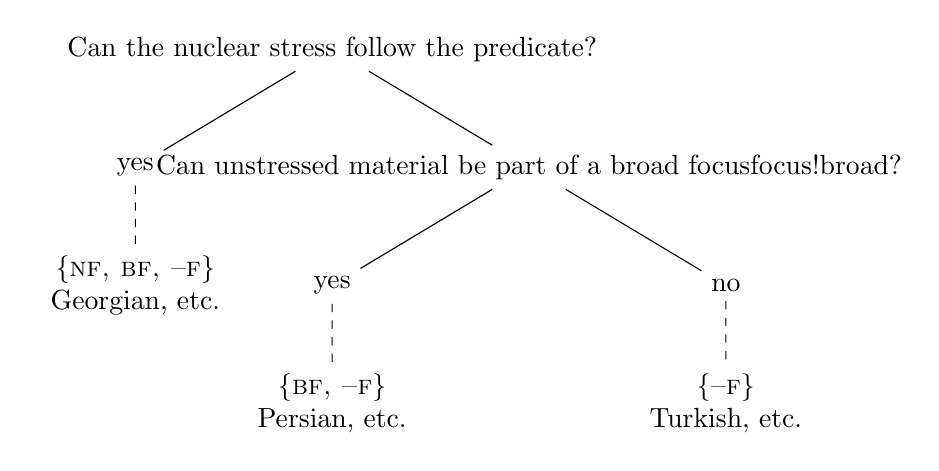
\begin{tikzpicture}
    \node {Can the nuclear stress follow the predicate?}[sibling distance = 5cm]
    child {node {yes}
    child {node {\parbox{2.5cm}{\centering \{\textsc{nf, bf, --f}\} \\ Georgian, etc.}} edge from parent [dashed]}}
    child {node {Can unstressed material be part of a broad focus\is{focus!broad}?}
    child {node {yes}
    child {node {\parbox{2cm}{\centering \{\textsc{bf, --f}\} \\ Persian, etc.}} edge from parent [dashed]}}
    child {node {no}
    child {node {\parbox{2cm}{\centering \{\textsc{--f}\} \\ Turkish, etc.}} edge from parent [dashed]}}
};
\end{tikzpicture}
\caption{Focus options of post-predicate objects by prosodic properties (\textsc{nf}: narrow focus\is{focus!narrow}; \textsc{bf}: broad focus, \textsc{--f}: out of focus)}
    \label{fig:treeProsody}
\end{figure}
The prosodic properties of the post-predicate domain offer a partial explanation of the cross-linguistic differences in \isi{focus} options in \figref{fig:treeIS}. In prosodic view, if post-predicate elements can host the nuclear stress, they can be used for (narrow/broad) \isi{focus}, as in Georgian\il{Kartvelian!Georgian}, Armenian, Caucasian Urum\il{Turkic!Caucasian Urum} and probably many Nakh-Daghestanian languages; see \figref{fig:treeProsody} and discussion about the languages in \sectref{sec:focusOptions}. If post-predicate elements cannot host the nuclear stress, then they cannot be narrowly focused, as in Persian\il{Persian}, Turkish\il{Turkic!Turkish}, Western Armenian\il{Armenian (Western)}. Within this group of languages, there is a further differentiation that cannot be accounted for by prosodic differences. In some languages (and at least at some level of meta-linguistic reflection), it is possible to use in broad focus\is{focus!broad} certain constructions with post-predicate elements that do not bear the nuclear stress (see discussion about Tsakhur and Persian\il{Persian} in \sectref{sec:focusOptions}). In Persian\il{Persian}, this possibility appears with nuclear stress on the verb, which applies to constructions with (preverbal/postverbal) specific objects (see \citealt[133--134]{modarresi_bare_2014} on Persian\il{Persian}). The nuclear stress must be hosted by the specific \isi{object} if it is in narrow \isi{focus} and it is exactly this \isi{focus} option that is banned from the post-predicate domain. This reasoning accounts for the facts from Persian\il{Persian}, but does not offer an explanation why the same flexibility does not hold true in Turkish\il{Turkic!Turkish}. The crucial issue is that there is nothing in the prosodic structure that would hinder a specific \isi{object} from being postverbal under broad focus\is{focus!broad} in these languages. Whether a language uses this construction (as Persian\il{Persian}) or not (as Turkish\il{Turkic!Turkish}) is an independent distinction that cannot be accounted for by \isi{prosody} alone.



\subsection{Prosody and postverbal narrow foci} 

Narrow foci come with an asymmetry in phrasing, such that preverbal foci are phrased together with the predicate, while postverbal foci are separated from the predicate with a prosodic break (see \sectref{sec:narrow}). This asymmetry follows from an independent phonological property of \isi{focus} in these languages, namely that the left edge of the \isi{focus} domain is aligned with a prosodic boundary, separating the \isi{focus} domain from the prefocal material (see \citealt{fery_focus_2013} for a typology in these lines). There is no evidence for a difference in the interpretation of preverbal and postverbal foci in languages that allow for both options: e.g., there is no difference in the interpretation of either option in Georgian\il{Kartvelian!Georgian}  \citep[]{skopeteas_Fanselow_focus_2010}.

An interesting question is whether the preference to align the left edge of the \isi{focus} with the left edge of a prosodic constituent (which applies to all examined languages) correlates with the evolution of a preverbal \isi{focus} position in these languages. If the underlying principle is to phrase the \isi{focus} together with the predicate, the prediction is straightforward: languages with an immediately-preverbal \isi{focus} are expected to insert a prosodic boundary at the left side of the \isi{focus} (see Georgian\il{Kartvelian!Georgian}, Eastern Armenian\il{Armenian (Eastern)} and Caucasian Urum\il{Turkic!Caucasian Urum} in \sectref{sec:narrow}), while languages with an immediately-postverbal \isi{focus} are expected to demarcate the \isi{focus} by means of a prosodic boundary on its right. Languages of the latter type are less frequent, but at least Zulu -- that has been the \isi{object} of extensive investigation in this respect -- confirms this prediction: narrow \isi{focus} is right adjacent to the predicate and the \isi{focus} is aligned with a boundary on its right \citep[]{cheng_against_2012}{}. However, there are various counterexamples to this putative generalization: various languages of India are reported to have preverbal foci and to align the right edge of the \isi{focus} with a prosodic boundary; see Bengali \citep[]{selkirk_bengali_2008}, Konkani \citep[709]{fery_focus_2013}. This left/right asymmetry suggests a bias towards aligning the left edge of the \isi{focus} with a prosodic boundary, which is not surprising: postfocal material is de-accented in most languages, which means that prosodic events following the \isi{focus} are less likely to appear in general.

\section*{Abbreviations}
\begin{tabularx}{.5\textwidth}{@{}lQ@{}}
3 & 3rd person\\
\textsc{acc} & {accusative}\\
\textsc{aor} & aorist\\
\textsc{caus} & causative\\
\textsc{dat} & {dative}\\
\textsc{def} & definite\\
\textsc{dem} & demonstrative\\
\textsc{erg} & {ergative}\\
\textsc{evid} & evidential\\
\textsc{io} & indirect object\is{object!indirect}\\
\textsc{nmlz} & nominalizer\\
\textsc{nom} & nominative\\
\end{tabularx}%
\begin{tabularx}{.5\textwidth}{@{}lQ@{}}
\textsc{pass} & passive\\
\textsc{pfv} & perfective\\
\textsc{pl} & plural\\
\textsc{poss} & possessor\\
\textsc{prog} & progressive\\
\textsc{pst} & past\\
\textsc{ra} & \textit{ra} (Persian)\\
\textsc{rem} & remote\\
\textsc{s} & subject\\
\textsc{sg} & singular\\
\textsc{sm} & series marker\\
\\
\end{tabularx}

\section*{Acknowledgements}
Grateful thanks to Deniz Balıkçıoğlu, Murat Baran, Hayk Hovhannisyan, Diana Kakashvili, Violeta Moisidi, Yasaman Sanei, and Saliha Seyis, who provided their intuitions and performed the illustrative sentences presented in this study. I am very grateful to the organizers Geoffrey Haig, Mohammad Rasekhmahand, Laurentia Schreiber, Nils Schiborr as well as the participants of the Workshop \textit{Post-predicate elements across the languages of Western Asia: theoretical and empirical approaches}  (September 22-23, 2022, University of Bamberg) for inspiring discussions on earlier versions of this study, as well as Hossep Dolatian and an anonymous reviewer for helpful comments.

\sloppy
\printbibliography[heading=subbibliography,notkeyword=this]
\end{document}
